\documentclass[tikz,border=2pt]{standalone}
\usepackage{lmodern}
\usepackage{amsmath,amssymb,bm}
\usetikzlibrary{arrows.meta,decorations.pathmorphing}
\definecolor{ink}{HTML}{1B2B37}
\definecolor{blue}{HTML}{087CAB}
\definecolor{orange}{HTML}{CE641B}
\definecolor{muted}{HTML}{596B77}
\definecolor{rule}{HTML}{D3DDE3}
\tikzset{
  column/.style={font=\sffamily\bfseries\fontsize{10}{12}\selectfont,text=ink},
  panel/.style={font=\sffamily\fontsize{9}{11}\selectfont,text=ink},
  label/.style={font=\fontsize{10}{12}\selectfont,text=ink},
  eq/.style={font=\fontsize{11}{13}\selectfont,text=ink},
  axis/.style={draw=muted!65,line width=.55pt,-{Latex[length=1.4mm]}},
  leg/.style={line width=.85pt,decorate,
    decoration={snake,amplitude=.55mm,segment length=3.1mm,
      pre length=1mm,post length=1mm}},
}
\begin{document}
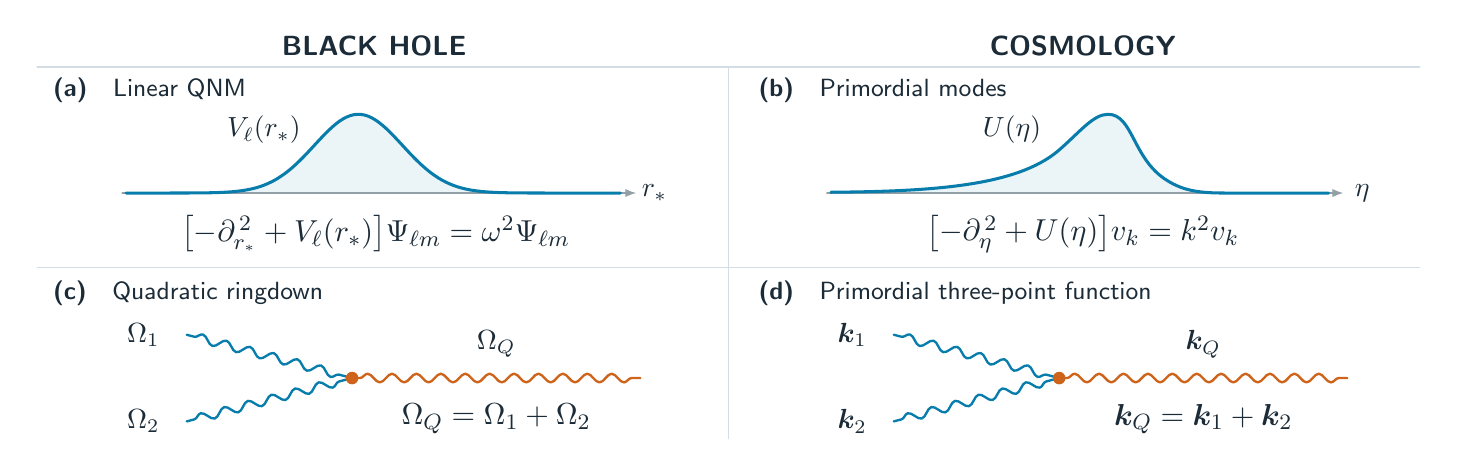
\begin{tikzpicture}[x=1cm,y=1cm,line cap=round,line join=round]
\useasboundingbox (0,.70) rectangle (17.8,6.0);
\node[column] at (4.4,5.77) {BLACK HOLE};
\node[column] at (13.4,5.77) {COSMOLOGY};
\draw[rule] (.12,5.50)--(17.68,5.50);
\draw[rule] (.12,2.95)--(17.68,2.95);
\draw[rule] (8.9,.78)--(8.9,5.50);

\node[panel,anchor=west] at (.20,5.20) {\textbf{(a)}\quad Linear QNM};
\node[panel,anchor=west] at (9.16,5.20) {\textbf{(b)}\quad Primordial modes};

\path[fill=blue!8] (1.25,3.90)
  plot[domain=1.25:7.53,samples=140]
    (\x,{3.90+1.0*exp(-((\x-4.20)/.79)^2)})
  --(7.53,3.90)--cycle;
\draw[axis] (1.20,3.90)--(7.73,3.90);
\draw[blue,line width=1.1pt,domain=1.25:7.53,samples=140]
  plot (\x,{3.90+1.0*exp(-((\x-4.20)/.79)^2)});
\node[label] at (3.00,4.70) {$V_\ell(r_*)$};
\node[label] at (7.96,3.90) {$r_*$};
\node[eq] at (4.42,3.38)
  {$\bigl[-\partial_{r_*}^{\,2}+V_\ell(r_*)\bigr]\Psi_{\ell m}
    =\omega^2\Psi_{\ell m}$};

\def\cosmopotential{
  (10.20,3.91)
  .. controls (11.50,3.92) and (12.55,3.99) .. (13.08,4.43)
  .. controls (13.36,4.67) and (13.53,4.90) .. (13.72,4.90)
  .. controls (14.04,4.90) and (14.03,4.33) .. (14.47,4.06)
  .. controls (14.69,3.92) and (14.91,3.90) .. (15.21,3.90)
  --(16.52,3.90)}
\path[fill=blue!8] \cosmopotential --(10.20,3.90)--cycle;
\draw[axis] (10.15,3.90)--(16.71,3.90);
\draw[blue,line width=1.1pt] \cosmopotential;
\node[label] at (12.50,4.70) {$U(\eta)$};
\node[label] at (16.95,3.90) {$\eta$};
\node[eq] at (13.40,3.38)
  {$\bigl[-\partial_\eta^{\,2}+U(\eta)\bigr]v_k=k^2v_k$};

\node[panel,anchor=west] at (.20,2.63) {\textbf{(c)}\quad Quadratic ringdown};
\node[panel,anchor=west] at (9.16,2.63) {\textbf{(d)}\quad Primordial three-point function};
\foreach \offset in {0,8.98}{
  \begin{scope}[shift={(\offset,0)}]
    \draw[leg,blue] (2.02,2.10)--(4.12,1.55);
    \draw[leg,blue] (2.02,1.00)--(4.12,1.55);
    \draw[leg,orange] (4.12,1.55)--(7.78,1.55);
    \fill[orange] (4.12,1.55) circle (.080);
  \end{scope}
}
\node[label,anchor=east] at (1.80,2.10) {$\Omega_1$};
\node[label,anchor=east] at (1.80,1.00) {$\Omega_2$};
\node[label] at (5.95,1.98) {$\Omega_Q$};
\node[eq] at (5.95,1.03) {$\Omega_Q=\Omega_1+\Omega_2$};
\node[label,anchor=east] at (10.78,2.10) {$\bm k_1$};
\node[label,anchor=east] at (10.78,1.00) {$\bm k_2$};
\node[label] at (14.93,1.98) {$\bm k_Q$};
\node[eq] at (14.93,1.03) {$\bm k_Q=\bm k_1+\bm k_2$};
\end{tikzpicture}
\end{document}
